\documentclass{../../slides-style}

\slidetitle[Лекция 1: Введение в робототехнику]{Алгоритмические основы робототехники}{17.02.2026}

\begin{document}

    \begin{frame}[plain]
        \titlepage
    \end{frame}

    \section{Организационное}

    \begin{frame}{Организационное}
        \begin{outline}
            \1 Семинары с одной вводной лекцией, две пары в неделю
            \1 В конце устный экзамен и аттестация по докладам
                \2 Два доклада на полчаса
                \2 Два вопроса без подготовки
            \1 Материалы лекций, темы докладов на \url{https://hwproj.ru/courses/50079}
            \1 Балльная система
                \2 5 баллов за доклад
                \2 10 баллов за экзамен
                \2 Итоговая оценка: $(\textrm{<сумма оценок>} -\ 5) * 10$
            \1 Коммуникации --- в чате потока
                \2 Также пишите в личку
        \end{outline}
    \end{frame}

    \begin{frame}{Зачем этот курс}
        \begin{outline}
            \1 Робототехника в общем смысле~--- очень перспективна
                \2 Беспилотные автомобили, БПЛА, \enquote{интернет вещей}
            \1 Курс~--- краткий обзор того, что вообще бывает, какая наука за этим стоит, чем можно заниматься в магистратуре
            \1 Немного общего низкоуровневого программирования, что никогда не лишне
            \1 Речь в основном про наземные мобильные роботы
            \1 Фокус на алгоритмике:
                \2 Не про паяльники и резьбу по дереву, не про теорию управления, не про искусственный интеллект
            \1 Кому нужны робототехники-программисты: \enquote{Сколтех}, ресурсный центр \enquote{Робототехника и БАС} СПбГУ, \enquote{Геоскан}, АО \enquote{Кама}, \enquote{Кибертех}, ЦНИИ РТК, \dots
        \end{outline}
    \end{frame}

    \begin{frame}{Что будет в курсе}
        \begin{outline}
            \1 Кинематика мобильного робота: виды и конфигурации колёс, \enquote{стандартная} трёхколёсная тележка, другие варианты кинематики (в т.ч. шагающие роботы)
            \1 Сенсорика: типы и физические принципы работы сенсоров, работа с ошибками измерений.
            \1 Отдельно видеокамеры, стереокамеры, сенсоры глубины
            \1 Алгоритмы машинного зрения, сегментация
            \1 Локализация, behavior-driven алгоритмы, belief representation, представление карты
            \1 SLAM
            \1 Планирование и \enquote{стратегическая} навигация
            \1 Аппаратные робототехнические платформы, от Arduino до KUKA
            \1 Программные платформы, ROS
        \end{outline}
    \end{frame}

    \section{Введение}

    \begin{frame}{Робототехника? Какая робототехника?}
        Робототехника --- наука об автономных технических системах, или о разработке и применении роботов.
        \begin{outline}
            \1 Слово \enquote{Робот} придумал Карел Чапек ещё в 1920
            \1 Часто под роботами понимают вообще автоматические машины для замены человека в труде
            \1 Следуя традициям СПбГУ, будем понимать под роботами таковые машины \emph{с обратной связью}
            \1 Есть ещё \emph{кибернетика} --- наука об управлении, раздел прикладной математики
        \end{outline}
    \end{frame}

    \begin{frame}{Какие роботы бывают}
        \begin{columns}
            \begin{column}{0.5\textwidth}
                \begin{outline}
                    \1 Стационарные (манипулятивные) роботы
                        \2 Промышленные роботы-манипуляторы
                        \2 Дельта-роботы
                    \1 Мобильные роботы
                        \2 Колёсные (гусеничные)
                        \2 БПЛА, подводные/надводные
                        \2 Шагающие
                \end{outline}
            \end{column}
            \begin{column}{0.5\textwidth}
                \begin{center}
                    \includegraphics[width=0.4\textwidth]{kuka.png}

                    \vspace{1cm}

                    \includegraphics[width=0.5\textwidth]{delta.png}
                \end{center}
            \end{column}
        \end{columns}
    \end{frame}

    \begin{frame}{Робототехника на матмехе}
        \begin{columns}
            \begin{column}{0.5\textwidth}
                \begin{outline}
                    \1 Образовательный конструктор ТРИК
                    \1 Среда программирования TRIK Studio/QReal:Robots
                    \1 Ресурсный центр \enquote{Робототехника и БАС}
                    \1 Кафедра теоретической кибернетики
                \end{outline}
            \end{column}
            \begin{column}{0.5\textwidth}
                \begin{center}
                    \includegraphics[width=0.6\textwidth]{trik.png}
                \end{center}
            \end{column}
        \end{columns}
    \end{frame}

    \section{Алгоритмические основы}

    \begin{frame}{Общая схема управления роботом}
        \framesubtitle{Sense-compute-control}
        \begin{center}
            \includegraphics[width=0.6\textwidth]{controlLoop.png}
            \attribution{R. Siegwart, I.R. Nourbakhsh, Introduction to Autonomous Mobile Robots}
        \end{center}
    \end{frame}

    \begin{frame}{Базовые схемы управления}
        \begin{outline}
            \1 Задача: имея установочное значение, вырабатывать управляющее воздействие так, чтобы система оставалась к установочному значению как можно ближе
            \1 Релейный регулятор: скачкообразное переключение управляющего воздействия при достижении порогового значения
            \1 Пропорциональный регулятор: управляющее воздействие пропорционально отклонению от установочного значения
            \1 Пропорционально-дифференциальный регулятор: управляющее воздействие пропорционально отклонению от установочного значения и скорости изменения отклонения
            \1 ПИД-регулятор: управляющее воздействие пропорционально всему выше и длительности отклонения
        \end{outline}
    \end{frame}

    \begin{frame}{Демо}
        \begin{center}
            \Huge{Демо на TRIK Studio}
        \end{center}
    \end{frame}

    \begin{frame}{Продвинутые подходы}
        \begin{columns}
            \begin{column}{0.5\textwidth}
                \begin{outline}
                    \1 Behavior-driven
                        \2 Условие-реакция
                        \2 Конечные автоматы
                        \2 Дерево поведений
                    \1 Локализация и планирование
                        \2 Локализация по ориентирам
                        \2 SLAM
                \end{outline}
            \end{column}
            \begin{column}{0.5\textwidth}
                \begin{center}
                    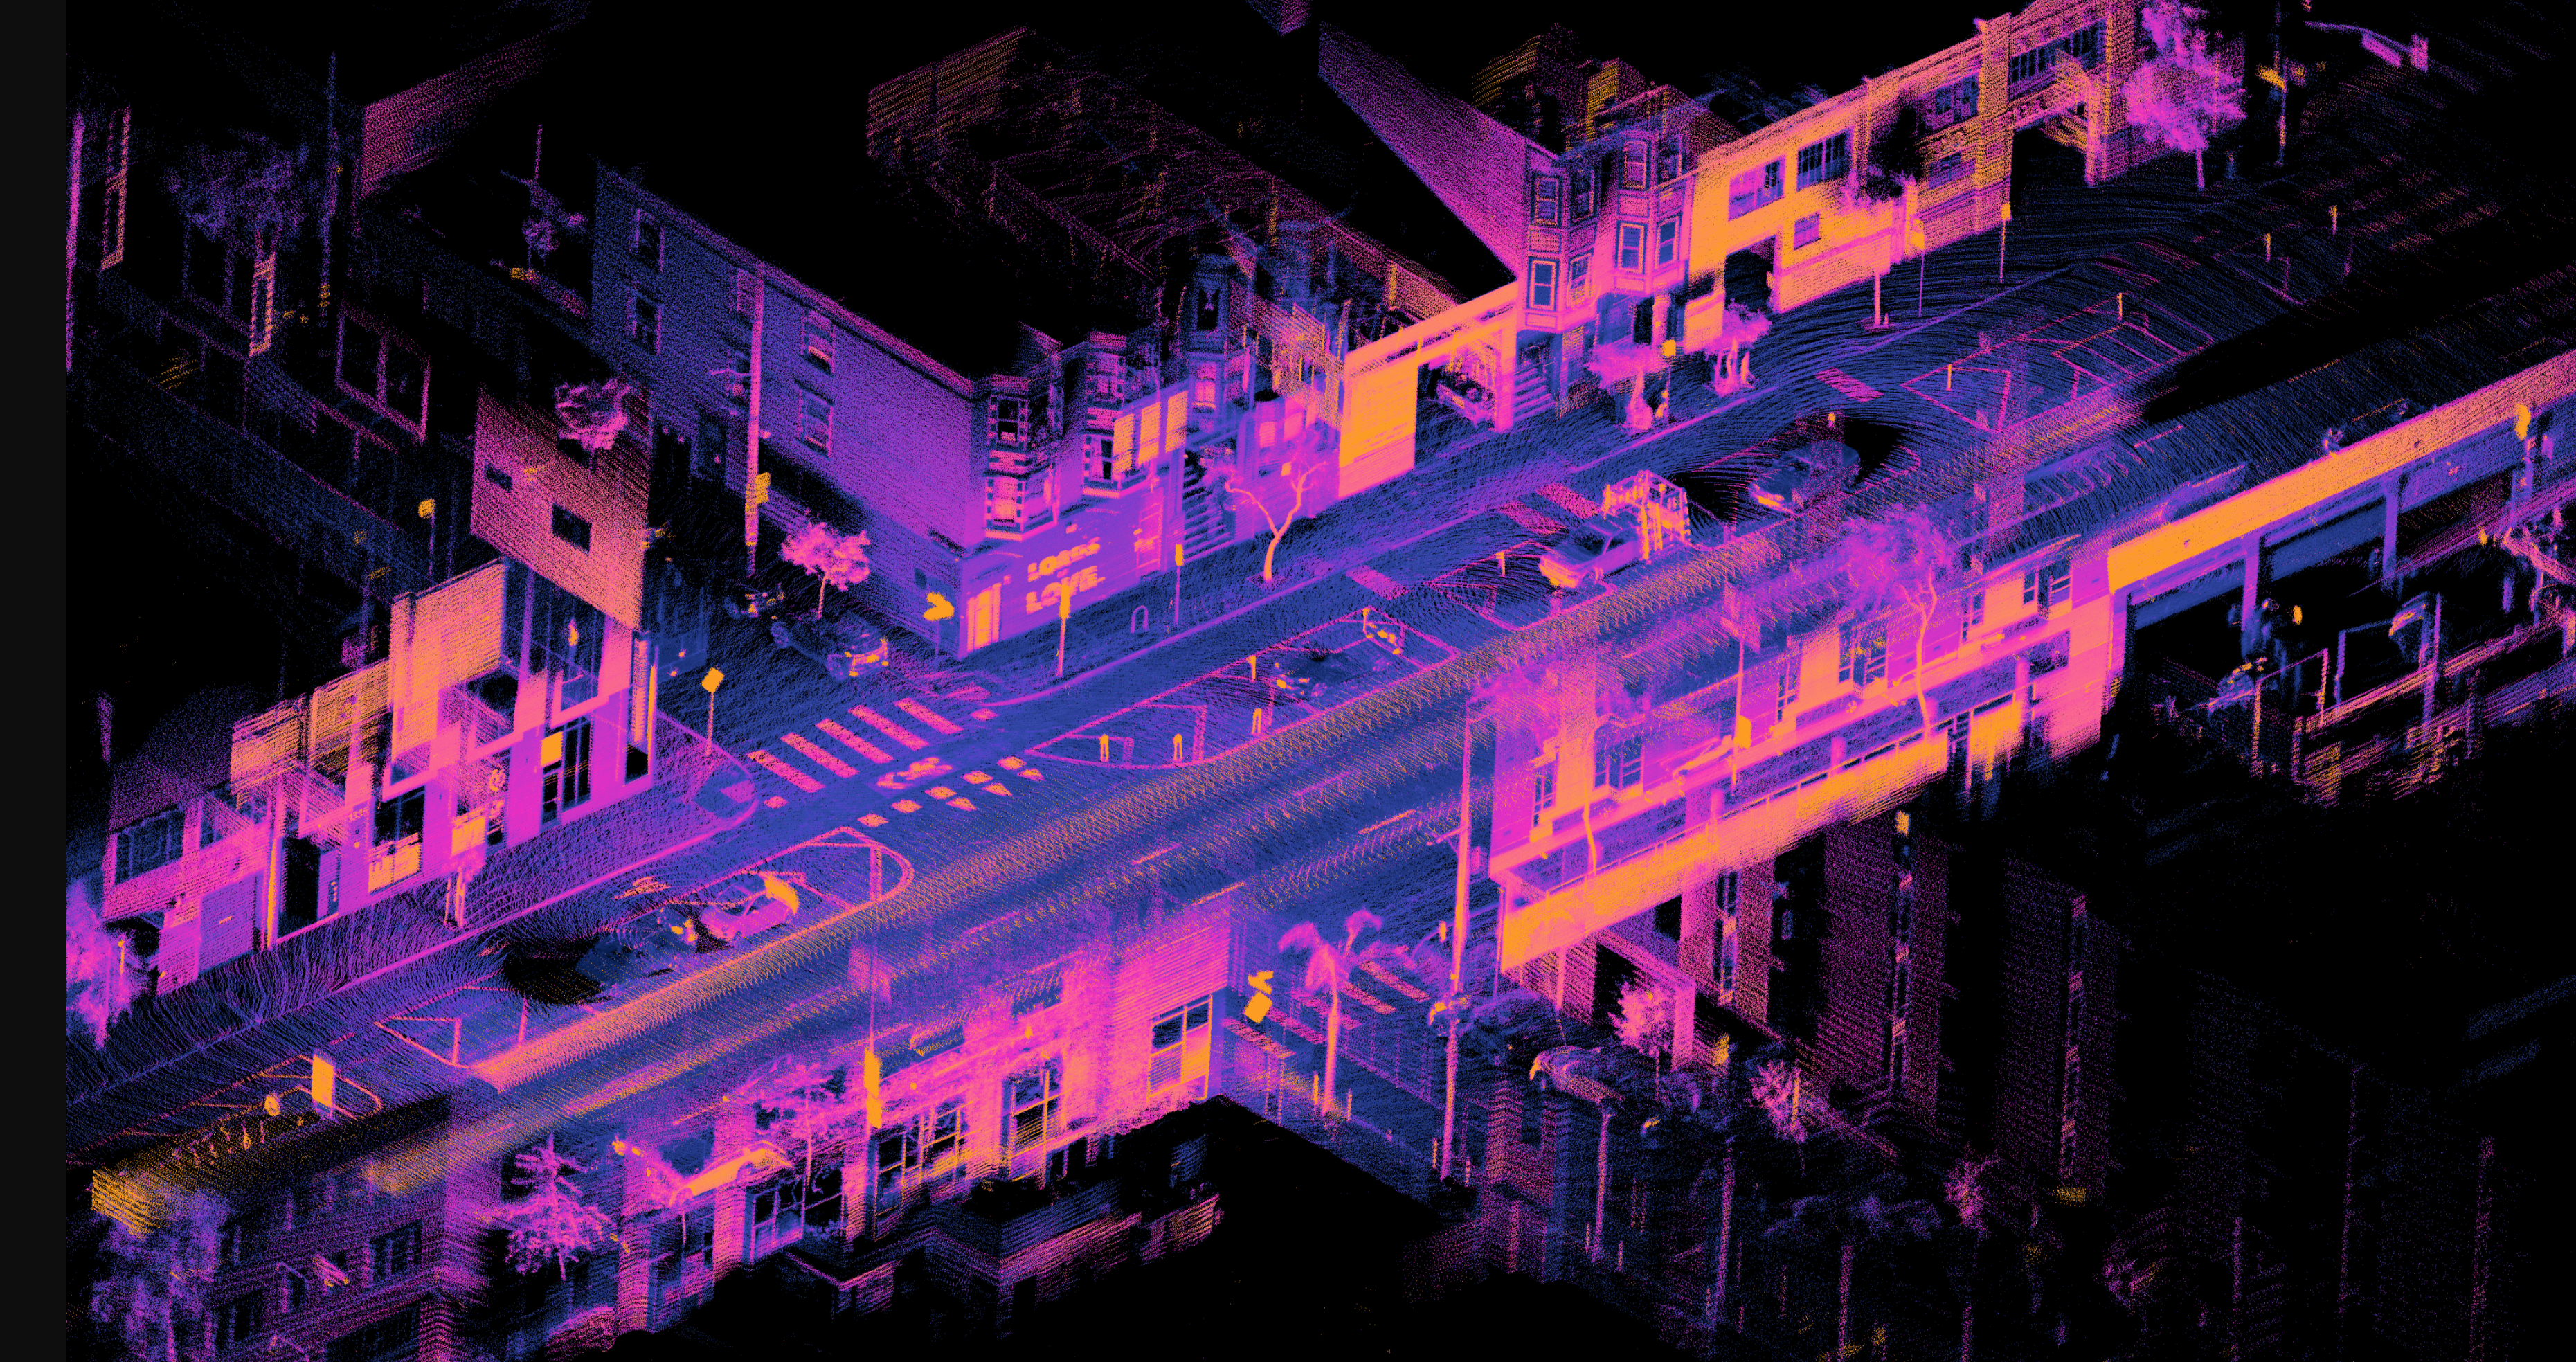
\includegraphics[width=0.9\textwidth]{slamMap.png}
                    \attribution{\url{https://en.wikipedia.org/wiki/Simultaneous_localization_and_mapping}}
                \end{center}
            \end{column}
        \end{columns}
    \end{frame}

    \section{Кинематика}

    \begin{frame}{Дьявол кроется в деталях}
        \framesubtitle{Кинематика робота}
        \begin{outline}
            \1 Виды задач
                \2 Прямая кинематическая задача --- есть модель и набор управляющих воздействий, какое положение робот займёт в пространстве?
                \2 Обратная кинематическая задача --- есть модель и целевое положение робота, каков набор управляющих воздействий?
            \1 Степени свободы --- сколько независимых параметров описывают состояние модели
                \2 Не всегда всеми ими можно управлять
                \2 Голономность
            \1 Модели:
                \2 Шагающие --- 2, 4, 6 ног
                \2 Колёсные --- четыре известных вида колеса, включая \enquote{шведские} и шар, более десятка известных конфигураций колёсных тележек
                    \3 \enquote{Автомобильное} управление (Аккермана), дифференциальное (\enquote{танковое}), омниколёса, \enquote{Synchro drive}
        \end{outline}
    \end{frame}

    \begin{frame}{Пример: синхропривод}
        \begin{center}
            \includegraphics[width=0.7\textwidth]{synchroDrive.png}
            \attribution{R. Siegwart, I.R. Nourbakhsh, Introduction to Autonomous Mobile Robots}
        \end{center}
    \end{frame}

    \begin{frame}{Поза робота}
        \framesubtitle{Для трёхколёсной дифференциальной тележки}
        \begin{columns}
            \begin{column}{0.6\textwidth}
                \begin{outline}
                    \1 Глобальная система координат
                    \1 Поза:
                        $$\xi_I = \begin{bmatrix} x \\ y \\ \theta \end{bmatrix}$$
                    \1 Прямая кинематическая модель:
                        $$\dot{\xi_I} = \begin{bmatrix} \dot{x} \\ \dot{y} \\ \dot{\theta} \end{bmatrix} = f(l, r, \theta, \dot{\phi_1}, \dot{\phi_2})$$
                    \1 Каждая модель накладывает ограничения на возможные движения
                \end{outline}
            \end{column}
            \begin{column}{0.4\textwidth}
                \begin{center}
                    \includegraphics[width=0.8\textwidth]{pose.png}
                    \attribution{R. Siegwart, I.R. Nourbakhsh, Introduction to Autonomous Mobile Robots}
                \end{center}
            \end{column}
        \end{columns}
    \end{frame}

    \begin{frame}{Задача управления}
        \begin{center}
            \includegraphics[width=0.7\textwidth]{inverseKinematics.png}
            \attribution{R. Siegwart, I.R. Nourbakhsh, Introduction to Autonomous Mobile Robots}
        \end{center}
    \end{frame}

    \section{Сенсорика}

    \begin{frame}{Виды сенсоров}
        \begin{outline}
            \1 Тактильные: кнопки, бамперы, неконтактные датчики
            \1 Энкодеры, разных видов: оптические, магнитные и т.п.
            \1 Датчики направления: компас, гироскоп, инклинометр
            \1 Датчики ориентиров: ГНСС, RF-метки и т.п.
            \1 Активные расстояния: УЗ, ИК, лазерные, радар, структурный свет
            \1 Движения/скорости: допплеровские радар или звуковые
            \1 Машинное зрение: камеры разных видов, стереопары, лидары
        \end{outline}
    \end{frame}

    \begin{frame}{Трудности}
        \begin{outline}
            \1 Шумы, фильтрация
                \2 Случайные и систематические ошибки
                \2 Скользящее среднее, медианный фильтр, фильтр Калмана
            \1 Sensor aliasing
            \1 Представление неопределённости
                \2 Одна гипотеза, несколько гипотез
            \1 Sensor fusion
            \1 Распространение ошибки
        \end{outline}
    \end{frame}

    \begin{frame}{Распространение ошибки}
        \begin{center}
            \includegraphics[width=0.7\textwidth]{poseUncertainity.png}
            \attribution{R. Siegwart, I.R. Nourbakhsh, Introduction to Autonomous Mobile Robots}
        \end{center}
    \end{frame}

    \begin{frame}{\enquote{Высокоуровневая} сенсорика}
        \begin{outline}
            \1 Depth from focus
            \1 Feature-based-стерео --- много разных алгоритмов сопоставления точек на кадрах с разных ракурсов
                \2 Дескриптор --- некое характерное представление точки, не зависящее от ракурса
            \1 Оптический поток (тоже feature-based), визуальная одометрия
            \1 Поиск границ, поиск геометрических примитивов
                \2 Лапласиан гауссиана, оператор Кэнни, преобразование Хафа
            \1 Сегментация, кластеризация (сейчас в основном машобуч)
                \2 DBSCAN, RANSAC
            \1 Whole-image features --- гистограммы, \enquote{отпечатки}
        \end{outline}
    \end{frame}

    \begin{frame}{Преобразование Хафа}
        \begin{center}
            \includegraphics[width=0.7\textwidth]{houghTransform.png}
            \attribution{\url{https://ru.wikipedia.org/wiki/Преобразование_Хафа}}
        \end{center}
    \end{frame}

    \begin{frame}{Общая схема сенсорики на CV}
        \begin{center}
            \includegraphics[width=0.7\textwidth]{cvScheme.png}
            \attribution{R. Siegwart, I.R. Nourbakhsh, Introduction to Autonomous Mobile Robots}
        \end{center}
    \end{frame}

    \section{Локализация}

    \begin{frame}{Задача навигации}
        Behavior-driven-навигация:
        \begin{center}
            \includegraphics[width=0.5\textwidth]{behaviorNavigation.png}
        \end{center}

        Навигация по карте:
        \begin{center}
            \includegraphics[width=0.5\textwidth]{mapBasedNavigation.png}
            \attribution{R. Siegwart, I.R. Nourbakhsh, Introduction to Autonomous Mobile Robots}
        \end{center}
    \end{frame}

    \begin{frame}{Определение положения}
        \begin{center}
            \includegraphics[width=0.9\textwidth]{uncertainity.png}
            \attribution{R. Siegwart, I.R. Nourbakhsh, Introduction to Autonomous Mobile Robots}
        \end{center}
    \end{frame}

    \begin{frame}{Belief representation}
        \begin{center}
            \includegraphics[width=0.45\textwidth]{beliefRepresentation.png}
            \attribution{R. Siegwart, I.R. Nourbakhsh, Introduction to Autonomous Mobile Robots}
        \end{center}
    \end{frame}

    \begin{frame}{Представление карты}
        \begin{columns}
            \begin{column}{0.5\textwidth}
                \begin{outline}
                    \1 Непрерывное --- геометрические примитивы
                    \1 Дискретное:
                        \2 Сетка
                        \2 Сетка с переменным размером ячейки
                        \2 Топологическое (в виде графа локаций)
                \end{outline}
            \end{column}
            \begin{column}{0.5\textwidth}
                \begin{center}
                    \includegraphics[width=0.8\textwidth]{variableCellGrid.png}
                    \attribution{R. Siegwart, I.R. Nourbakhsh, Introduction to Autonomous Mobile Robots}
                \end{center}
            \end{column}
        \end{columns}
    \end{frame}

    \begin{frame}{Локализация}
        \begin{outline}
            \1 Инерциальная навигация, проприоцепция
            \1 Локализация по ориентирам
            \1 Марковская --- поддерживаем набор предположений о том, где мы, уточняем по сенсорам
            \1 Фильтр Калмана --- оптимизируем предсказанное положение робота и данные сенсоров
            \1 Simultaneous Localization And Mapping --- строим карту и пытаемся определить своё положение на ней
        \end{outline}
    \end{frame}

    \begin{frame}{Схема локализации фильтром Калмана}
        \begin{center}
            \includegraphics[width=0.6\textwidth]{kalmanLocalization.png}
            \attribution{R. Siegwart, I.R. Nourbakhsh, Introduction to Autonomous Mobile Robots}
        \end{center}
    \end{frame}

    \begin{frame}{Схема SLAM}
        \begin{center}
            \includegraphics[width=0.65\textwidth]{slam.png}
            \attribution{R. Siegwart, I.R. Nourbakhsh, Introduction to Autonomous Mobile Robots}
        \end{center}
    \end{frame}

    \begin{frame}{Проблема замыкания траектории}
        \begin{center}
            \includegraphics[width=0.7\textwidth]{slamErrors.png}
            \attribution{R. Siegwart, I.R. Nourbakhsh, Introduction to Autonomous Mobile Robots}
        \end{center}
    \end{frame}

    \section{Навигация}

    \begin{frame}{Задача навигации}
        \begin{outline}
            \1 Задача: зная карту и своё положение на ней, достичь позиции (или группы позиций) $p$ в момент времени не позже $n$
            \1 Но есть нюансы:
                \2 Мы достигаем не позиции $p$, а состояния, в котором верим, что достигли позиции $p$, то есть строим траекторию не по карте, а по нашим представлениям
                \2 Как правило, мы не знаем точной карты
                \2 Карта может меняться со временем
                    \3 Задача обхода препятствий
            \1 integrated planning and execution
        \end{outline}
    \end{frame}

    \begin{frame}{Слоистая архитектура системы навигации}
        \begin{columns}
            \begin{column}{0.5\textwidth}
                \begin{center}
                    \includegraphics[width=0.7\textwidth]{navigationLayers.png}
                \end{center}
            \end{column}
            \begin{column}{0.5\textwidth}
                \begin{center}
                    \includegraphics[width=0.7\textwidth]{navigationTiers.png}
                \end{center}
            \end{column}
        \end{columns}
        \attribution{R. Siegwart, I.R. Nourbakhsh, Introduction to Autonomous Mobile Robots}
    \end{frame}

    \section{Программно-инженерные аспекты}

    \begin{frame}{Аппаратные платформы}
        \begin{columns}
            \begin{column}{0.55\textwidth}
                \begin{outline}
                    \1 Готовые роботы --- KUKA
                    \1 Платы \enquote{сделай сам} --- Arduino в различных вариациях, Raspberry Pi, \dots
                    \1 Образовательные/платформы для прототипирования --- ТРИК, Vex, Fishertechnik
                \end{outline}
            \end{column}
            \begin{column}{0.45\textwidth}
                \begin{center}
                    \includegraphics[width=0.6\textwidth]{arduinoUno.png}
                    \attribution{R. Siegwart, I.R. Nourbakhsh, Introduction to Autonomous Mobile Robots}
                \end{center}
            \end{column}
        \end{columns}
    \end{frame}

    \begin{frame}{Симуляторы}
        \begin{columns}
            \begin{column}{0.5\textwidth}
                \begin{outline}
                    \1 Player/Stage/Gazebo
                    \1 Webots
                    \1 CoppeliaSim (бывший V-REP)
                    \1 Microsoft AirSim
                \end{outline}
            \end{column}
            \begin{column}{0.5\textwidth}
                \begin{center}
                    \includegraphics[width=0.8\textwidth]{airSim.png}
                    \attribution{https://microsoft.github.io/AirSim}
                \end{center}
            \end{column}
        \end{columns}
    \end{frame}

    \begin{frame}{Программные платформы}
        \begin{columns}
            \begin{column}{0.4\textwidth}
                \begin{outline}
                    \1 ROS/ROS2
                    \1 Player
                    \1 RT-middleware
                    \1 YARP
                \end{outline}
            \end{column}
            \begin{column}{0.6\textwidth}
                \begin{center}
                    \includegraphics[width=0.9\textwidth]{ros.png}
                    \attribution{\url{https://www.researchgate.net/figure/Comparison-between-ROS-and-ROS2_fig4_335382592}}
                \end{center}
            \end{column}
        \end{columns}
    \end{frame}

    \section{Заключение}

    \begin{frame}{Книжка}
        \begin{columns}
            \begin{column}{0.5\textwidth}
                Roland Siegwart, Illah Reza Nourbakhsh, Introduction to Autonomous Mobile Robots, MIT Press, 2004, 321 pages
            \end{column}
            \begin{column}{0.5\textwidth}
                \begin{center}
                    \includegraphics[width=0.7\textwidth]{bookCover.png}
                \end{center}
            \end{column}
        \end{columns}
    \end{frame}

\end{document}
